\section{Среда разработки аппаратуры QReal:HaSCoL}
Технология QReal:HaSCoL была исторически первой технологией, разработанной автором 
на платформе QReal, и именно опыт её разработки во многом определил направления дальнейших 
исследований и, в итоге, полученные в данной диссертации результаты. В частности, 
в ходе этой работы возникла потребность в визуальном метаредакторе. Данная технология 
не использует многих описанных в этой работе возможностей платформы QReal, поскольку 
на момент работы над ней эти возможности ещё не были реализованы, кроме того, сведения, 
приведённые в обзоре аналогичных подходов, могли устареть. Это не представляется критичным 
недостатком, поскольку основная цель дальнейшего изложения --- продемонстрировать 
пример разработки предметно-ориентированного визуального языка, причём для данной 
работы более важны методологические аспекты, чем специфика предметной области или особенности реализации конкретной DSM-платформы. 
% TODO: Убрать?
В этом плане предлагаемый пример интересен тем, что язык создавался и был строго формализован как расширение метамодели 
языка UML 2.0, поэтому данный опыт может быть использован для сравнения с более "`легковесными"' 
подходами, применявшимися в примерах из разделов~\ref{chapter:qRealRobots} и~\ref{chapter:qRealUbiq}.

\subsection{Постановка задачи}
Различные встроенные устройства играют большую роль в нашей жизни, однако задача их 
разработки всё ещё остаётся сложной и трудоёмкой. В 80-х годах двадцатого века появились языки Verilog и VHDL%
%TODO: Сноски
, которые и по сей день остаются фактическим стандартом в деле разработки аппаратного 
обеспечения. Эти языки позволяют описать устройство аналогично коду обычной программы, 
их синтаксис похож на синтаксис традиционных языков программирования. Они позволяют 
синтезировать описание разрабатываемого аппаратного обеспечения, пригодное для производства, 
или произвести эмуляцию.

Тем не менее, данные языки заставляют описывать систему в низкоуровневых терминах, 
поэтому актуальна задача разработки новых технологий с более высоким уровнем абстракции. 
Визуальные методы разработки в данной предметной области даже более применимы, чем 
в области разработки ПО, поскольку аппаратное обеспечение традиционно описывалось 
различными чертежами и схемами. Однако же, в силу высокой (и постоянно растущей) сложности 
аппаратного обеспечения, средство визуального моделирования не может быть просто редактором 
электронных схем, а должно само поддерживать высокоуровневые концепции. Ещё одним 
важным требованием, накладываемым на такое средство, является исполнимость модели. 
Средство должно иметь возможность синтезировать описание устройства в виде, пригодном 
для использования промышленным оборудованием при производстве, и генерировать эмулятор 
устройства, позволяющий вести отладку, тестирование и оценку производительности, не 
прибегая к созданию дорогостоящего прототипа. Все эти сложности затрудняют разработку 
новых визуальных технологий.

На кафедре системного программирования математико-механического факультета СПбГУ разрабатывается 
текстовый язык разработки аппаратных систем HaSCoL (Hardware-Software Codesign Language)
% TODO: [ссылки], http://oops.math.spbu.ru/projects/coolkit
гораздо более высокого уровня, чем VHDL или Verilog. Перед автором данной диссертации 
была поставлена задача разработать визуальную технологию, которая бы использовала 
язык HaSCoL как целевой язык для генерации и позволяла бы проектировать аппаратуру 
в высокоуровневых терминах этого языка. Это дало бы возможность использовать инструментальные 
средства HaSCoL для создания как спецификации устройства для конфигурации FPGA
% TODO: Сноска
или производства, так и для генерации программного эмулятора. С другой стороны, визуальная 
технология должна была повысить удобство программирования на языке HaSCoL, а поскольку 
этот язык новый, это могло бы позитивно сказаться на эффективности его внедрения. 
Кроме того, использование высокоуровневого языка в качестве целевого для генерации 
свело бы к минимуму затраты на анализ предметной области при разработке DSM-решения, 
поскольку большая часть этой работы уже была выполнена при разработке текстового языка.

Язык HaSCoL описывает систему  в терминах исполняемых параллельно обработчиков сигналов.
Обработчики объединены в процессы --- сущности, инкапсулирующие в себе ресурсы (данные), 
обработчики сигналов и другие процессы, и имеющие входы и выходы. Обработчик представляет 
из себя последовательность однотактовых шагов, выполняющихся, если некоторые условия 
(получение сообщения, состояние ресурсов процесса) истинны. Обработчики могут начинать 
своё исполнение на каждом такте, на котором выполнены условия его старта, вне зависимости 
от того, выполняются они уже или нет. Пример описания процесса%
%TODO (из работы [ссылка])
:

\vspace{5mm}
\begin{minipage}{\linewidth}
\begin{verbatim}
process DynamicArbiter =
begin
  in one(uint(2), uint(8));
  in two(uint(2), uint(8));
  out res(uint(8));
  group {
    -- что делать, если пришли оба сигнала:
    -- условия на принимаемые сигналы определяют готовность
    -- принятия данных из каждого входа в отдельности
    one(prio1, data1) and prio1 >= prio2,
    two(prio2, data2) and prio1 < prio2
    {
      send res (if prio1 >= prio2 then data1 else data2 fi)
    }
   -- если пришел только один сигнал --- случай попроще
   -- подчеркивание вместо имени параметра означает, что
   -- нас данный параметр не интересует и пользоваться им
   -- мы не будем
    one(_, ddata) {send res (ddata)}
    two(_, ddata) {send res (ddata)}
  }
end
\end{verbatim}
\end{minipage}
\vspace{5mm}

Процесс имеет два входа (one, two) с двумя параметрами и выход res, возвращающий значение 
типа uint(8). Конструкцией group три обработчика объединены в группу, перед фигурными 
скобками записано условие, при истинности которого обработчик начнёт работу, внутри 
фигурных скобок --- тело обработчика. В условиях могут участвовать проверки наличия 
данных на входах, логические выражения с участием входных данных и локальных данных 
процесса. Конструкция send в теле обработчика --- посылка сигнала на указанный выход. 
Входы и выходы могут также иметь несколько портов, каждый порт может быть связан с 
очередью сообщений. Например,

\begin{verbatim}
in InputData (int(16))[A[1], B];
\end{verbatim}
определяет вход с одним параметром и двумя портами, при этом размер очереди порта 
A --- 1, размер очереди порта B --- 0.

Для поддержки структурной декомпозиции процессов в язык был введён структурный уровень. 
Структурные конструкции позволяют отображать входы объемлющего процесса на порты входов 
вложенного, и выходы вложенного процесса на выходы объемлющего или входы вложенного, 
позволяя таким образом структурно декомпозировать процессы на наборы взаимодействующих 
вложенных подпроцессов.

Каждый процесс имеет свой тип, задаваемый явно или неявно. Тип процесса --- перечень 
его входов и выходов с указанием типов их аргументов. Над типами процессов определено 
отношение структурного сабтайпинга --- неформально говоря, процесс A имеет тип, являющийся 
подтипом типа процесса B, если A можно везде использовать вместо B. Тип процесса по 
умолчанию получается из спецификации процесса, тип можно указать и явно, это используется, 
например, для описания свойств параметров функторов.

Функтор --- это процесс, параметризованный другим процессом. Например,

\vspace{5mm}
\begin{minipage}{\linewidth}
\begin{verbatim}
process Wrapper (P: Proc) =
begin
  process X = P;
  process Y = P;
  ...
end
\end{verbatim}
\end{minipage}
\vspace{5mm}

Процесс Wrapper параметризован процессом P типа Proc. Применение функтора выглядит так:
\begin{verbatim}
process W = Wrapper(aProc);
\end{verbatim}

\subsection{Существующие средства визуального описания аппаратных систем}
Самый известный из существующих визуальных языков, UML 2, создавался с учётом необходимости 
описывать аппаратные средства. В версиях UML 1.x специальных средств для описания 
аппаратных систем не было, поэтому приходилось создавать профили UML, например, UML-RT.
% TODO: ссылка 
В UML 2 этот пробел был заполнен, в язык было введено понятие "`структурированный классификатор"', 
который может содержать внутри себя набор частей, соединённых между собой соединителями. 
Взаимодействие структурированных классификаторов с внешним миром и внутренними частями 
происходит исключительно через порты. Порт --- это точка взаимодействия со строго 
определённым интерфейсом. Один структурированный классификатор может иметь несколько 
портов, а также имеет возможность определить, на какой из портов пришёл запрос. Запросы, 
приходящие на порты, могут быть обработаны непосредственно объектом-хозяином порта 
или переданы на порт какой-либо его части. Каждый порт имеет набор предоставляемых 
им интерфейсов и набор интерфейсов, требуемых от внешней среды. Пример нотации представлен 
на рисунке~\ref{image:umlStructuredClassifier}.

\begin{figure} [ht]
	\begin{center}
		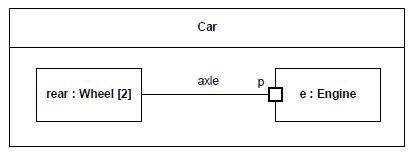
\includegraphics[width=0.6\textwidth]{appendixA/A.3/umlStructuredClassifier.png}
		\caption{Структурированный классификатор UML 2.}
		\label{image:umlStructuredClassifier}
	\end{center}
\end{figure}

Для задания внутреннего поведения элементов системы в UML 2 обычно используется диаграмма 
конечных автоматов. Каждый структурированный классификатор может иметь связанный с 
ним конечный автомат, который описывает реакцию на события, приходящие на его порты.

Помимо "`чистого"' UML 2 используются и специальные профили UML, предназначенные для 
использования с текстовыми языками (подход, весьма близкий к предлагаемому). Пример 
такого профиля --- 
% TODO: представленный в работе [ссылка] 
профиль UML для языка SystemC. SystemC
% TODO [ссылка] 
--- язык проектирования уровня системы, основанный на C++ и поддерживаемый группой крупных компаний. 
% TODO: Каких?
Система в SystemC состоит из модулей, каждый модуль может содержать переменные, порты 
для взаимодействия с окружением и процессы, реализующие функциональность модуля. Процессы
исполняются параллельно и могут реагировать на события. Связь между модулями осуществляется 
с помощью портов, которые предоставляют модулям доступ к каналам. Каналы бывают примитивными 
и иерархическими: иерархический канал --- тоже модуль, имеет свои процессы и может иметь 
доступ к другим каналам.

Профиль UML для SystemC логически разделён на 3 части.
\begin{enumerate}
	\item Структуры и коммуникации --- определяет стереотипы для базовых строительных 
		блоков SystemC. Эти стереотипы представляют модули, порты, интерфейсы и каналы, 
		и используются на различных диаграммах UML, например, на диаграммах классов и 
		диаграммах композитных структур.
	\item Поведение и синхронизация --- определяет стереотипы для спецификации поведения 
		процессов SystemC. Эти стереотипы используются в диаграммах состояний UML.
	\item Типы данных --- представляет типы данных SystemC.
\end{enumerate}

Пример нотации профиля UML для SystemC представлен на рисунке~\ref{image:systemCExample}.

\begin{figure} [ht]
	\begin{center}
		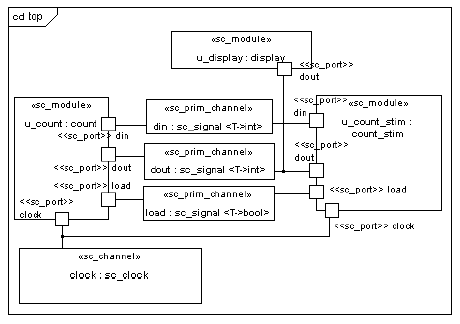
\includegraphics[width=0.8\textwidth]{appendixA/A.3/systemCExample.png}
		\caption{Пример нотации профиля для SystemC.}
		\label{image:systemCExample}
	\end{center}
\end{figure}

Как видно из обзора, идея визуального моделирования аппаратного обеспечения не нова, 
при этом наибольшее внимание уделяется языку UML (по-видимому, как наиболее распространённому 
визуальному языку). При этом, существующие языки пытаются целиком специфицировать 
систему графическими средствами, что зачастую приводит к весьма громоздким диаграммам.

\subsection{Предлагаемый набор визуальных языков}
Основные принципы, в соответствии с которыми разрабатывалась нотация, таковы.
\begin{enumerate}
	\item Модель должна быть исполняемой, то есть позволять синтезировать код на языке 
		системы CoolKit без необходимости ручной корректировки результатов. Пригодная 
		для промышленного использования технология должна позволять программисту получать 
		готовую низкоуровневую спецификацию системы или эмулятор, действуя в одной среде 
		разработки и, желательно, с одним представлением системы.
	\item Графическими примитивами должны быть представлены только те элементы программы, 
		которые наиболее выгодно представлять графически. Остальная необходимая для синтеза 
		информация должна быть представлена на визуальной модели в текстовой форме. Такой 
		подход позволяет сохранять диаграммы достаточно компактными, но при этом, как 
		обсуждалось в разделе~\ref{chapter:qRealUbiq}, делает программы существенно более 
		сложными для понимания.
	\item Нотация разрабатывалась для использования внутри среды разработки, поэтому 
		некоторые её элементы могут быть неудобны для представления на бумаге.
\end{enumerate}

Для визуализации языка CoolKit плохо подходит непосредственно UML и даже профиль для 
UML --- целевой язык не является строго говоря объектно-ориентированным, к тому же 
обладает рядом особенностей, которые плохо или неудобно выражаются в терминах UML. 
Предлагаемый графический язык, хотя и не является профилем UML, сформулирован с активным 
использованием метамодели UML. Для формализации языка используется метамоделирование 
на метаязыке MOF --- синтаксис графических конструкций языка описан с помощью диаграмм UML. 
Метамодель языка построена на метамодели ядра и некоторых диаграмм UML, таким образом, 
язык лишь незначительно отличается от UML, и его синтаксис и семантика интуитивно понятны 
специалистам, занимающимся визуальным моделированием. Кроме того, переиспользование 
метамодели UML позволило сэкономить массу усилий при формализации языка. Одним из 
полученных результатов стало понимание того, что формализация предметно-ориентированных 
языков программирования может быть существенно упрощена благодаря переиспользованию 
некоей стандартной метамодели, например, UML.

Для спецификации системы в нашем языке используется два вида диаграмм --- диаграмма 
типов процессов и диаграмма отображения портов. Заметим, что мы избежали необходимости 
использовать диаграммы автоматов для описания поведения системы --- эту роль выполняют 
текстовые блоки на целевом языке. Диаграмма типов процессов базируется на диаграмме 
классов UML, а диаграмма отображения портов --- на диаграмме композитных структур.

\subsubsection{Диаграмма типов процессов}
Диаграмма типов процессов используется для задания основных структурных свойств и 
отношений процессов, составляющих пакет или приложение. На диаграмме изображаются сами 
процессы, их входы и выходы, отношения вложенности, отношения генерализации, и функторы. 
Заметим, что на этой диаграмме не рисуются обработчики событий, и могут не рисоваться 
ресурсы процесса (список ресурсов процесса может быть неполным, из того, что ресурс 
не изображён на диаграмме, нельзя делать вывод, что он не описан в процессе). Некоторые 
вложенные процессы тоже могут быть опущены на этой диаграмме, если это не повлияет 
на корректность модели. Часть метамодели диаграммы представлена на рисунке~\ref{image:processTypesMetamodel}.

\begin{figure} [ht]
	\begin{center}
		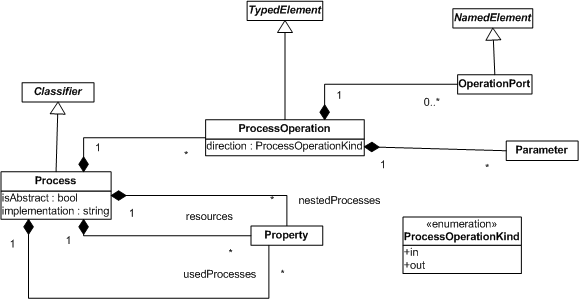
\includegraphics[width=0.9\textwidth]{appendixA/A.3/processTypesMetamodel.png}
		\caption{Метамодель диаграммы типов процессов.}
		\label{image:processTypesMetamodel}
	\end{center}
\end{figure}

Пример изображения вложенных процессов представлен на рисунке~\ref{image:processTypesNotation}. 
Как видно из примера, нотация перечисляет ресурсы, входы и выходы процессов в таком 
виде, в каком они были в языке системы CoolKit. По-настоящему графически здесь изображаются 
только отношения использования одного процесса внутри другого или вложенности процессов 
(т.е. когда один процесс описан непосредственно внутри другого). Заметим, что вложенный 
процесс может не иметь имени --- тогда оно просто не отображается на диаграмме. Поскольку 
вложенные или используемые процессы являются деталями реализации объемлющего процесса, 
они могут не рисоваться на диаграмме. 

\begin{figure} [ht]
	\begin{center}
		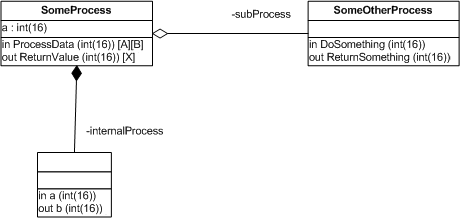
\includegraphics[width=0.7\textwidth]{appendixA/A.3/processTypesNotation.png}
		\caption{Нотация процессов.}
		\label{image:processTypesNotation}
	\end{center}
\end{figure}

Существенную выгоду от использования этого типа диаграммы можно получить при использовании 
в программе функторов. Пример нотации объявления функторов приведён на рисунке~\ref{image:functorsNotation}. 

\begin{figure} [ht]
	\begin{center}
		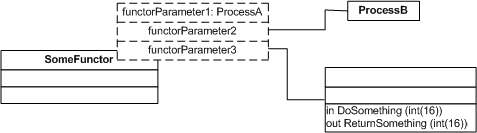
\includegraphics[width=0.7\textwidth]{appendixA/A.3/functorsNotation.png}
		\caption{Нотация функторов.}
		\label{image:functorsNotation}
	\end{center}
\end{figure}

В частности, из-за особенности нотации, которую можно видеть на примере, было принято 
решение не использовать диаграммы классов UML. Нотация отражает возможность языка 
системы CoolKit описывать тип процесса --- формальный параметр функтора прямо в месте 
описания формального параметра. Вынесение типов параметров в отдельные графические 
сущности позволяет сделать отношения между процессами --- формальными или фактическими 
параметрами функторов гораздо более наглядными. Применение функтора изображается так, 
как показано на рисунке~\ref{image:functorApplication}.

\begin{figure} [ht]
	\begin{center}
		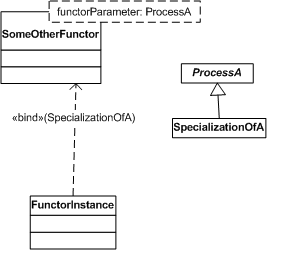
\includegraphics[width=0.5\textwidth]{appendixA/A.3/functorApplication.png}
		\caption{Применение функтора.}
		\label{image:functorApplication}
	\end{center}
\end{figure}

Для того, чтобы проиллюстрировать применение диаграммы типов процессов, рассмотрим 
содержательный пример --- задачу об арбитре динамических приоритетов 4 в 1%
%TODO: из [ссылка] 
. Задача формулируется следующим образом: на один из четырёх входов поступают данные, 
первый параметр пришедших данных --- приоритет. Если в одном такте данные поступили 
на несколько входов, на выход выдаются данные с наибольшим приоритетом, остальные 
входы объявляются неготовыми. Если приходит только одно сообщение, оно отправляется 
на выход.

Следуя оригинальному решению поступим следующим образом --- сначала напишем арбитр 
динамических приоритетов 2 в 1 (с двумя входами и одним выходом), затем создадим арбитр-функтор 
4 в 1, использующий 3 арбитра 2 в 1, который и решит задачу (см. рисунок~\ref{image:arbiter4To1ProcessTypes}). 

\begin{figure} [ht]
	\begin{center}
		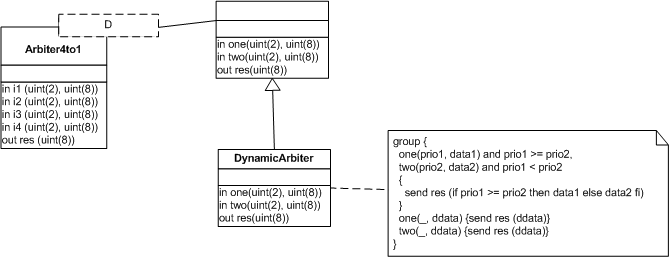
\includegraphics[width=\textwidth]{appendixA/A.3/arbiter4To1ProcessTypes.png}
		\caption{Диаграмма типов процессов для задачи "`Арбитр 4 в 1"'.}
		\label{image:arbiter4To1ProcessTypes}
	\end{center}
\end{figure}

В комментарии --- код процесса DynamicArbiter на языке системы CoolKit, описывающий 
реализацию арбитра 2 к 1. Код из комментария при синтезе добавляется к сгенерированному 
описанию процесса, таким образом мы получаем полностью специфицированный арбитр 2 к 1, 
который может быть использован как фактический параметр функтора Arbiter4to1 (на это 
указывает отношение генерализации, связывающее DynamicArbiter и безымянный тип процесса --- 
формальный параметр функтора). Про процесс Arbiter4to1 мы указали пока только то, 
что он является функтором (готов использовать любой процесс, поддерживающий интерфейс 
арбитра 2 к 1, который мы определили с помощью безымянного типа процесса), и указали, 
что у него есть 4 входа и один выход --- то есть просто "нарисовали" условие задачи.

\subsubsection{Диаграмма отображения портов}
Диаграмма отображения портов рисуется для отдельного процесса и используется для отображения 
связей между входными и выходными портами вложенных процессов того процесса, для которого 
рисовалась диаграмма. Таким образом, эта диаграмма фактически является графической 
нотацией для структурного уровня языка системы CoolKit. Синтаксис с незначительными 
изменениями совпадает с синтаксисом диаграммы составных структур UML. На диаграмме 
изображаются процессы и их порты (все порты входов и выходов), связи между портами, 
внутри процессов могут находиться вложенные процессы. Важно различие между процессом 
верхнего уровня --- процессом, относительно которого рисуется диаграмма, и вложенными 
процессами. Вложенные процессы на самом деле являются экземплярами процессов, имеют 
имя и тип. Процесс верхнего уровня имеет только тип. Пример нотации изображён на рисунке~\ref{image:portMappingsExample}. 
Вернёмся к нашему примеру с арбитром 4 к 1. Диаграмма отображения портов для этого примера 
выглядит так, как показано на рисунке~\ref{image:arbiter4To1PortMappings}.

\begin{figure} [ht]
	\begin{center}
		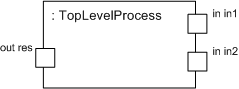
\includegraphics[width=0.4\textwidth]{appendixA/A.3/portMappingsExample.png}
		\caption{Процесс на диаграмме отображения портов.}
		\label{image:portMappingsExample}
	\end{center}
\end{figure}

\begin{figure} [ht]
	\begin{center}
		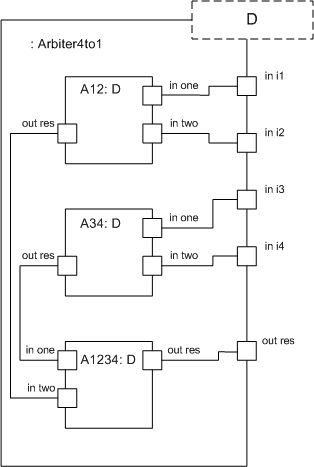
\includegraphics[width=0.5\textwidth]{appendixA/A.3/arbiter4To1PortMappings.png}
		\caption{Диаграмма отображения портов для задачи "`Арбитр 4 в 1"'.}
		\label{image:arbiter4To1PortMappings}
	\end{center}
\end{figure}

Здесь мы видим процесс верхнего уровня Arbiter4to1 --- без имени, но с типом и с формальным 
параметром функтора. Arbiter4to1 имеет 4 входных порта и 1 выходной, их типы здесь 
уже можно не указывать, они были на диаграмме типов процессов, которую мы нарисовали 
ранее. Процесс имеет три вложенных процесса A12, A34 и A1234 типа D, который, как 
следует из диаграммы типов процессов, описывает процессы, имеющие два входа и один 
выход. Если мы считаем, что в качестве параметра функтора передаётся арбитр 2 к 1, 
изображённое на рисунке соединение портов решает задачу.

\subsubsection{Генерация}
Генерация в язык системы CoolKit проходит довольно очевидным образом, поскольку графический 
и текстовый языки имеют одинаковую модель представления аппаратного устройства. Скелеты 
описаний процессов генерируются по диаграмме типов процессов, потом они дополняются 
вложенными процессами и конструкциями, описывающими связь портов по диаграмме отображения 
портов, потом они дополняются реализацией, которая так или иначе представлена в текстовом 
виде на диаграмме --- в виде комментария или в виде неотображаемого атрибута процесса. 
В результате получается полная программа на языке системы CoolKit, готовая к дальнейшей 
трансляции в VHDL и далее --- в эмулятор или спецификацию устройства.

При генерации считается, что одноимённые однотипные сущности в одном пространстве 
имён представляют собой одну сущность. То есть, например, если на одной диаграмме 
описан процесс с одним входом, а на другой диаграмме описан процесс с тем же именем 
и другим входом, будет сгенерирован один процесс с двумя входами. Такой подход позволяет 
изображать на каждой диаграмме только существенные для неё части системы, хотя и может 
привести к некоторой сложности для понимания набора диаграмм в целом. Предполагается, 
что у средства визуального моделирования существует возможность удобным способом предоставить 
пользователю информацию о невидимых на диаграмме элементах. Есть некоторые тонкости 
с тем, что разные формально сущности на разных диаграммах представляют собой одну 
логическую сущность, например, процесс на диаграмме типов процессов и процесс на диаграмме 
отображения портов. Такие сущности всё же должны считаться генерацией однотипными и 
объединяться в одну сущность. Например, двух ранее приведённых диаграмм, описывающих 
реализацию арбитра 4 к 1, достаточно, чтобы сгенерировать такой код на языке системы CoolKit:

\vspace{5mm}
\begin{minipage}{\linewidth}
\begin{verbatim}
process DynamicArbiter =
begin
  in one(uint(2), uint(8));
  in two(uint(2), uint(8));
  out res(uint(8));
  group {
    one(prio1, data1) and prio1 >= prio2,
    two(prio2, data2) and prio1 < prio2
    {
      send res (if prio1 >= prio2 then data1 else data2 fi)
    }
    one(_, ddata) {send res (ddata)}
    two(_, ddata) {send res (ddata)}
  }
end

process Arbiter4to1 (D : begin
  in one(uint(2), uint(8));
  in two(uint(2), uint(8));
  out res(uint(8));
  end
) =
begin
  in i1 (uint(2), uint(8));
  in i2 (uint(2), uint(8));
  in i3 (uint(2), uint(8));
  in i4 (uint(2), uint(8));
  out res (uint(8));
  process A12 = D with one = i1, two = i2, res = A1234.one;
  process A34 = D with one = i3, two = i4, res = A1234.two;
  process A1234 = D with res = res;
end
\end{verbatim}
\end{minipage}
\vspace{5mm}

Для того, чтобы получить исполнимый код, нужно создать экземпляр процесса Arbiter4to1, 
использующий в качестве параметра процесс DynamicArbiter. Для этого достаточно нарисовать 
диаграмму, изображённую на рисунке~\ref{image:arbiter4To1FunctorApplication}.

\begin{figure} [ht]
	\begin{center}
		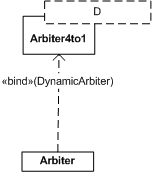
\includegraphics[width=0.2\textwidth]{appendixA/A.3/arbiter4To1FunctorApplication.png}
		\caption{Применение функтора "`Арбитр 4 к 1"'.}
		\label{image:arbiter4To1FunctorApplication}
	\end{center}
\end{figure}

Эта диаграмма породит код 

\begin{verbatim}
process Arbiter = Arbiter4to1(DynamicArbiter);
\end{verbatim}

Этот код вместе с приведённым ранее кодом может быть синтезирован и исполнен на эмуляторе.

\subsection{Результаты проекта QReal:HaSCoL}
В результате работы над технологией QReal:Hascol было создано два языка, с помощью 
которых описывалась структурная часть системы. Технология не была доведена до промышленного 
использования, полученные результаты нигде не публиковались, связано это с недостаточной 
зрелостью базовой технологии QReal на момент работы над QReal:HaSCoL. Однако проблемы, 
возникшие при разработке, во многом послужили мотивацией для реализации тех возможностей 
метатехнологии QReal, которые представляются в данной работе. Кроме того, визуальный язык 
QReal:HaSCoL далее использовался как пример для апробации различных новых возможностей 
QReal, например, "`метамоделирования на лету"'~\cite{takun2011diploma, ptakhina2013course}.

С точки зрения введённой в данной работе классификации созданные языки являются статическими 
текстовографическими языками. В данном случае использование текстовой нотации не так 
осложняет понимание диаграмм, как в случае QReal:Ubiq (раздел~\ref{chapter:qRealUbiq}), 
поскольку текстовая и графическая части не взаимозаменяемы: структурная часть системы 
целиком описывается графически, поведенческая --- целиком текстово. Были предприняты 
попытки использовать диаграммы активностей языка UML 2.0 для задания и поведенческой 
части в графическом виде, но в результате получались громоздкие и трудночитаемые диаграммы, 
поэтому было принято решение поведенческую часть задавать в текстовом виде.

В отличие от всех последующих языков на базе платформы QReal, языки QReal:HaSCoL создавались 
на базе метамодели UML 2.0. Это было сделано для того, чтобы строго формализовать 
язык и сделать возможной его реализацию не только на базе QReal (впрочем, таких попыток 
не предпринималось), а также опробовать на реальном примере такой подход к разработке 
синтаксиса языка. Результаты показали, что переиспользование метамодели UML действительно 
позволяет сэкономить много усилий (потребовалось ввести всего две-три новые сущности 
на каждый язык из семейства), однако от разработчика требуется хорошо ориентироваться
в метамодели UML, что само по себе весьма непросто. Стандарт UML достаточно объёмен, 
а метамодель весьма запутанна (особую сложность для читаемости метамодели представляет 
активное использование операций объединения пакетов PackageMerge и использование сущностей 
с одинаковыми именами в разных пакетов). Как кажется, затраты на изучение метамодели 
UML превышают выгоду, получаемую от переиспользования этой метамодели, так что разрабатывать 
новый предметно-ориентированный язык "`с нуля"' с использованием метаязыка выбранной 
DSM-платформы более оправданно, чем перед созданием языка специально изучать метамодель 
UML. Наличие эффективных инструментальных средств, помогающих разобраться в больших 
метамоделях наподобие UML и автоматизировать переиспользование фрагментов метамодели, 
как кажется, смогло бы изменить ситуацию, однако на данный момент такие средства не 
распространены, и создание таких средств представляется интересным направлением дальнейших 
исследований.
